\RequirePackage[l2tabu, orthodox]{nag}
\documentclass[version=3.21, pagesize, twoside=off, bibliography=totoc, DIV=calc, fontsize=12pt, a4paper, french, english]{scrartcl}
%Permits to copy eg x ⪰ y ⇔ v(x) ≥ v(y) from PDF to unicode data, and to search. From pdfTeX users manual. See https://tex.stackexchange.com/posts/comments/1203887.
	\input glyphtounicode
	\pdfgentounicode=1
%Latin Modern has more glyphs than Computer Modern, such as diacritical characters. fntguide commands to load the font before fontenc, to prevent default loading of cmr.
	\usepackage{lmodern}
%Encode resulting accented characters correctly in resulting PDF, permits copy from PDF.
	\usepackage[T1]{fontenc}
%UTF8 seems to be the default in recent TeX installations, but not all, see https://tex.stackexchange.com/a/370280.
	\usepackage[utf8]{inputenc}
%Provides \newunicodechar for easy definition of supplementary UTF8 characters such as → or ≤ for use in source code.
	\usepackage{newunicodechar}
%Text Companion fonts, much used together with CM-like fonts. Provides \texteuro and commands for text mode characters such as \textminus, \textrightarrow, \textlbrackdbl.
	\usepackage{textcomp}
%St Mary’s Road symbol font, used for ⟦ = \llbracket. The \SetSymbolFont command avoids spurious warnings, but also some valid ones, see https://tex.stackexchange.com/a/106719/.
	%\usepackage{stmaryrd}\SetSymbolFont{stmry}{bold}{U}{stmry}{m}{n}
%Solves bug in lmodern, https://tex.stackexchange.com/a/261188; probably useful only for unusually big font sizes; and probably better to use exscale instead. Note that the authors of exscale write against this trick.
	%\DeclareFontShape{OMX}{cmex}{m}{n}{
		%<-7.5> cmex7
		%<7.5-8.5> cmex8
		%<8.5-9.5> cmex9
		%<9.5-> cmex10
	%}{}
	%\SetSymbolFont{largesymbols}{normal}{OMX}{cmex}{m}{n}
%More symbols (such as \sum) available in bold version, see https://github.com/latex3/latex2e/issues/71. In article mode (but not in presentation mode), also hides some potentially useful warnings such as when using $\bm{\llbracket}$, see stmaryrd in this document (not sure why).
	\DeclareFontShape{OMX}{cmex}{bx}{n}{%
	   <->sfixed*cmexb10%
	   }{}
	\SetSymbolFont{largesymbols}{bold}{OMX}{cmex}{bx}{n}
%https://english.stackexchange.com/questions/93008
	\usepackage[super]{nth}
%For small caps also in italics, see https://tex.stackexchange.com/questions/32942/italic-shape-needed-in-small-caps-fonts, https://tex.stackexchange.com/questions/284338/italic-small-caps-not-working.
	\usepackage{slantsc}
	\AtBeginDocument{%
		%“Since nearly no font family will contain real italic small caps variants, the best approach is to substitute them by slanted variants.” -- slantsc doc
		%\DeclareFontShape{T1}{lmr}{m}{scit}{<->ssub*lmr/m/scsl}{}%
		%There’s no bold small caps in Latin Modern, we switch to Computer Modern for bold small caps, see https://tex.stackexchange.com/a/22241
		%\DeclareFontShape{T1}{lmr}{bx}{sc}{<->ssub*cmr/bx/sc}{}%
		%\DeclareFontShape{T1}{lmr}{bx}{scit}{<->ssub*cmr/bx/scsl}{}%
	}
%Warn about missing characters.
	\tracinglostchars=2
%Nicer tables: provides \toprule, \midrule, \bottomrule.
	%\usepackage{booktabs}
%For new column type X which stretches; can be used together with booktabs, see https://tex.stackexchange.com/a/97137. “tabularx modifies the widths of the columns, whereas tabular* modifies the widths of the inter-column spaces.” Loads array.
	%\usepackage{tabularx}
%math-mode version of "l" column type. Requires \usepackage{array}.
	%\usepackage{array}
	%\newcolumntype{L}{>{$}l<{$}}
%Provides \xpretocmd and loads etoolbox which provides \apptocmd, \patchcmd, \newtoggle… Also loads xparse, which provides \NewDocumentCommand and similar commands intended as replacement of \newcommand in LaTeX3 for defining commands (see https://tex.stackexchange.com/q/98152 and https://github.com/latex3/latex2e/issues/89).
	\usepackage{xpatch}
%ntheorem doc says: “empheq provides an enhanced vertical placement of the endmarks”; must be loaded before ntheorem. Loads the mathtools package, which loads and fixes some bugs in amsmath and provides \DeclarePairedDelimiter. amsmath is considered a basic, mandatory package nowadays (Grätzer, More Math Into LaTeX).
	\usepackage[ntheorem]{empheq}
%Package frenchb asks to load natbib before babel-french. Package hyperref asks to load natbib before hyperref.
	\usepackage{natbib}

\newtoggle{LCpres}
	\newtoggle{LCart}
	\newtoggle{LCposter}
	\makeatletter
	\@ifclassloaded{beamer}{
		\toggletrue{LCpres}
		\togglefalse{LCart}
		\togglefalse{LCposter}
		\wlog{Presentation mode}
	}{
		\@ifclassloaded{tikzposter}{
			\toggletrue{LCposter}
			\togglefalse{LCpres}
			\togglefalse{LCart}
			\wlog{Poster mode}
		}{
			\toggletrue{LCart}
			\togglefalse{LCpres}
			\togglefalse{LCposter}
			\wlog{Article mode}
		}
	}
	\makeatother%

%Language options ([french, english]) should be on the document level (last is main); except with tikzposter: put [french, english] options next to \usepackage{babel} to avoid warning. beamer uses the \translate command for the appendix: omitting babel results in a warning, see https://github.com/josephwright/beamer/issues/449. Babel also seems required for \refname.
	\iftoggle{LCpres}{
		\usepackage{babel}
	}{
	}
	%\frenchbsetup{AutoSpacePunctuation=false}
%listings (1.7) does not allow multi-byte encodings. listingsutf8 works around this only for characters that can be represented in a known one-byte encoding and only for \lstinputlisting. Other workarounds: use literate mechanism; or escape to LaTeX (but breaks alignment).
	%\usepackage{listings}
	%\lstset{tabsize=2, basicstyle=\ttfamily, escapechar=§, literate={é}{{\'e}}1}
%I favor acro over acronym because the former is more recently updated (2018 VS 2015 at time of writing); has a longer user manual (about 40 pages VS 6 pages if not counting the example and implementation parts); has a command for capitalization; and acronym suffers a nasty bug when ac used in section, see https://tex.stackexchange.com/q/103483 (though this might be the fault of the silence package and might be solved in more recent versions, I do not know) and from a bug when used with cleveref, see https://tex.stackexchange.com/q/71364. However, loading it makes compilation time (one pass on this template) go from 0.6 to 1.4 seconds, see https://bitbucket.org/cgnieder/acro/issues/115.
	\usepackage[single]{acro}
	\DeclareAcronym{AMCD}{short=AMCD, long={Aide Multicritère à la Décision}}
\DeclareAcronym{AHP}{short=AHP, long={Analytic Hierarchy Process}}
\DeclareAcronym{AR}{short=AR, long={Argumentative Recommender}}
\DeclareAcronym{DA}{short=DA, long={Decision Analysis}}
\DeclareAcronym{DJ}{short=DJ, long={Deliberated Judgment}}
\DeclareAcronym{DM}{short=DM, long={Decision Maker}}
\DeclareAcronym{DP}{short=DP, long={Deliberated Preference}}
\DeclareAcronym{MAVT}{short=MAVT, long={Multiple Attribute Value Theory}}
\DeclareAcronym{MCDA}{short=MCDA, long={Multicriteria Decision Aid}}
\DeclareAcronym{MIP}{short=MIP, long={Mixed Integer Program}}
\DeclareAcronym{SEU}{short=SEU, long={Subjective Expected Utility}}


\iftoggle{LCpres}{
	%I favor fmtcount over nth because it is loaded by datetime anyway; and fmtcount warns about possible conflicts when loaded after nth.
	\usepackage{fmtcount}
	%For nice input of date of presentation. Must be loaded after the babel package. Has possible problems with srcletter: https://golatex.de/verwendung-von-babel-und-datetime-in-scrlttr2-schlaegt-fehlt-t14779.html.
	\usepackage[nodayofweek]{datetime}
}{
}
%For presentations, Beamer implicitely uses the pdfusetitle option. ntheorem doc says to load hyperref “before the first use of \newtheorem”. autonum doc mandates option hypertexnames=false. I want to highlight links only if necessary for the reader to recognize it as a link, to reduce distraction. In presentations, this is already taken care of by beamer (https://tex.stackexchange.com/a/262014). If using colorlinks=true in a presentation, see https://tex.stackexchange.com/q/203056. Crashes the first compilation with tikzposter, just compile again and the problem disappears, see https://tex.stackexchange.com/q/254257.
\makeatletter
\iftoggle{LCpres}{
	\usepackage{hyperref}
}{
	\usepackage[hypertexnames=false, pdfusetitle, linkbordercolor={1 1 1}, citebordercolor={1 1 1}, urlbordercolor={1 1 1}]{hyperref}
	%https://tex.stackexchange.com/a/466235
	\pdfstringdefDisableCommands{%
		\let\thanks\@gobble
	}
}
\makeatother
%urlbordercolor is used both for \url and \doi, which I think shouldn’t be colored, and for \href, thus might want to color manually when required. Requires xcolor.
	\NewDocumentCommand{\hrefblue}{mm}{\textcolor{blue}{\href{#1}{#2}}}
%hyperref doc says: “Package bookmark replaces hyperref’s bookmark organization by a new algorithm (...) Therefore I recommend using this package”.
	\usepackage{bookmark}
%Need to invoke hyperref explicitly to link to line numbers: \hyperlink{lintarget:mylinelabel}{\ref*{lin:mylinelabel}}, with \ref* to disable automatic link. Also see https://tex.stackexchange.com/q/428656 for referencing lines from another document.
	%\usepackage{lineno}
	%\NewDocumentCommand{\llabel}{m}{\hypertarget{lintarget:#1}{}\linelabel{lin:#1}}
	%\setlength\linenumbersep{9mm}
%For complex authors blocks. Seems like authblk wants to be later than hyperref, but sooner than silence. See https://tex.stackexchange.com/q/475513 for the patch to hyperref pdfauthor.
	\ExplSyntaxOn
	\seq_new:N \g_oc_hrauthor_seq
	\NewDocumentCommand{\addhrauthor}{m}{
		\seq_gput_right:Nn \g_oc_hrauthor_seq { #1 }
	}
	%Should be \NewExpandableDocumentCommand, but this is not yet provided by my version of xparse
	\DeclareExpandableDocumentCommand{\hrauthor}{}{
		\seq_use:Nn \g_oc_hrauthor_seq {,~}
	}
	\ExplSyntaxOff
	{
		\catcode`#=11\relax
		\gdef\fixauthor{\xpretocmd{\author}{\addhrauthor{#2}}{}{}}%
	}
	\iftoggle{LCart}{
		\usepackage{authblk}
		\renewcommand\Affilfont{\small}
		\fixauthor
		\AtBeginDocument{
		    \hypersetup{pdfauthor={\hrauthor}}
		}
	}{
	}
%I do not use floatrow, because it requires an ugly hack for proper functioning with KOMA script (see scrhack doc). Instead, the following command centers all floats (using \centering, as the center environment adds space, http://texblog.net/latex-archive/layout/center-centering/), and I manually place my table captions above and figure captions below their contents (https://tex.stackexchange.com/a/3253).
	\makeatletter
	\g@addto@macro\@floatboxreset\centering
	\makeatother
%Permits to customize enumeration display and references
	%\nottoggle{LCpres}{
		%\usepackage{enumitem} %follow list environments by a string to customize enumeration, example: \begin{description}[itemindent=8em, labelwidth=!] or \begin{enumerate}[label=({\roman*}), ref={\roman*}].
	%}{
	%}
%Provides \Centering, \RaggedLeft, and \RaggedRight and environments Center, FlushLeft, and FlushRight, which allow hyphenation. With tikzposter, seems to cause 1=1 to be printed in the middle of the poster.
	%\usepackage{ragged2e}
%To typeset units by closely following the “official” rules.
	%\usepackage[strict]{siunitx}
%Turns the doi provided by some bibliography styles into URLs. However, uses old-style dx.doi url (see 3.8 DOI system Proxy Server technical details, “Users may resolve DOI names that are structured to use the DOI system Proxy Server (https://doi.org (current, preferred) or earlier syntax http://dx.doi.org).”, https://www.doi.org/doi_handbook/3_Resolution.html). The patch solves this.
	\usepackage{doi}
	\makeatletter
	\patchcmd{\@doi}{http://dx.doi.org}{https://doi.org}{}{}
	\makeatother
%Makes sure upper case greek letters are italic as well.
	\usepackage{fixmath}
%Provides \mathbb; obsoletes latexsym (see http://tug.ctan.org/macros/latex/base/latexsym.dtx). Relatedly, \usepackage{eucal} to change the mathcal font and \usepackage[mathscr]{eucal} (apparently equivalent to \usepackage[mathscr]{euscript}) to supplement \mathcal with \mathscr. This last option is not very useful as both fonts are similar, and the intent of the authors of eucal was to provide a replacement to mathcal (see doc euscript). Also provides \mathfrak for supplementary letters.
	\usepackage{amsfonts}
%Provides a beautiful (IMHO) \mathscr and really different than \mathcal, for supplementary uppercase letters. But there is no bold version. Alternative: mathrsfs (more slanted), but when used with tikzposter, it warns about size substitution, see https://tex.stackexchange.com/q/495167.
	\usepackage[scr]{rsfso}
%Multiple means to produce bold math: \mathbf, \boldmath (defined to be \mathversion{bold}, see fntguide), \pmb, \boldsymbol (all legacy, from LaTeX base and AMS), \bm (the most recommended one), \mathbold from package fixmath (I don’t see its advantage over \boldsymbol).
%“The \boldsymbol command is obtained preferably by using the bm package, which provides a newer, more powerful version than the one provided by the amsmath package. Generally speaking, it is ill-advised to apply \boldsymbol to more than one symbol at a time.” — AMS Short math guide. “If no bold font appears to be available for a particular symbol, \bm will use ‘poor man’s bold’” — bm. It is “best to load the package after any packages that define new symbol fonts” – bm. bm defines \boldsymbol as synonym to \bm. \boldmath accesses the correct font if it exists; it is used by \bm when appropriate. See https://tex.stackexchange.com/a/10643 and https://github.com/latex3/latex2e/issues/71 for some difficulties with \bm.
	\usepackage{bm}
	\nottoggle{LCpres}{
	%https://ctan.org/pkg/amsmath recommends ntheorem, which supersedes amsthm, which corrects the spacing of proclamations and allows for theoremstyle. Option standard loads amssymb and latexsym. Must be loaded after amsmath (from ntheorem doc). From cleveref doc, “ntheorem is fully supported and even recommended”; says to load cleveref after ntheorem. When used with tikzposter, warns about size substitution for the lasy (latexsym) font when using \url, because ntheorem loads latexsym; relatedly (but not directly related to ntheorem), size substitution warning with the cmex font happens when loading amsmath and using \url. According to https://tex.stackexchange.com/q/535950, ntheorem “seems essentially unmaintaned and has severe problems”, but I use it anyway because it is very handy. Yields “! LaTeX Error: Something's wrong--perhaps a missing \item.” if some theorem follows thebibliography.
		\usepackage[thmmarks, amsmath, standard, hyperref]{ntheorem}
		%empheq doc says to do this after loading ntheorem
		\usetagform{default}
	%Provides \cref. Unfortunately, cref fails when the language is French and referring to a label whose name contains a colon (https://tex.stackexchange.com/q/83798). Use \cref{sec\string:intro} to work around this. cleveref should go “laster” than hyperref.
		\usepackage{cleveref}
	}{
	}
	\nottoggle{LCposter}{
	%Equations get numbers iff they are referenced. Loading order should be “amsmath → hyperref → cleveref → autonum”, according to autonum doc. Use this in preference to the showonlyrefs option from mathtools, see https://tex.stackexchange.com/q/459918 and autonum doc. See https://tex.stackexchange.com/a/285953 for the etex line. Incompatible with my version of tikzposter (produces “! Improper \prevdepth”).
		\expandafter\def\csname ver@etex.sty\endcsname{3000/12/31}\let\globcount\newcount
		\usepackage{autonum}
	}{
	}
%Also loaded by tikz.
	%\usepackage{xcolor}
\iftoggle{LCpres}{
	\usepackage{tikz}
	%\usetikzlibrary{babel, matrix, fit, plotmarks, calc, trees, shapes.geometric, positioning, plothandlers, arrows, shapes.multipart}
}{
}
%Vizualization, on top of TikZ
	%\usepackage{pgfplots}
	%\pgfplotsset{compat=1.14}
\usepackage{graphicx}
	\graphicspath{{graphics/}}

%Provides \printlength{length}, useful for debugging.
	%\usepackage{printlen}
	%\uselengthunit{mm}

\iftoggle{LCpres}{
	\usepackage{appendixnumberbeamer}
	%I have yet to see anyone actually use these navigation symbols; let’s disable them
	\setbeamertemplate{navigation symbols}{} 
	\usepackage{preamble/beamerthemeParisFrance}
	\setcounter{tocdepth}{10}
}{
}

%Do not use the displaymath environment: use equation. Do not use the eqnarray or eqnarray* environments: use align(*). This improves spacing. (See l2tabu or amsldoc.)


%Requires package xcolor.
\definecolor{ao(english)}{rgb}{0.0, 0.5, 0.0}
\NewDocumentCommand{\commentOC}{m}{\textcolor{blue}{\small$\big[$OC: #1$\big]$}}
%Requires package babel and option [french]. According to babel doc, need two braces around \selectlanguage to make the changes really local.
\NewDocumentCommand{\commentOCf}{m}{\textcolor{blue}{{\small\selectlanguage{french}$\big[$OC : #1$\big]$}}}
\NewDocumentCommand{\commentPB}{m}{\textcolor{red}{{\small\selectlanguage{french}$\big[$PB : #1$\big]$}}}
\NewDocumentCommand{\commentRT}{m}{\textcolor{ao(english)}{{\small\selectlanguage{french}$\big[$RT : #1$\big]$}}}

\bibliographystyle{abbrvnat}
\NewDocumentCommand{\possessivecite}{mO{}}{\citeauthor{#1}’s \citeyearpar[#2]{#1}}

\newtheorem{conjecture}{Conjecture}

%https://tex.stackexchange.com/a/467188, https://tex.stackexchange.com/a/36088 - uncomment if one of those symbols is used.
%\DeclareFontFamily{U} {MnSymbolD}{}
%\DeclareFontShape{U}{MnSymbolD}{m}{n}{
%  <-6> MnSymbolD5
%  <6-7> MnSymbolD6
%  <7-8> MnSymbolD7
%  <8-9> MnSymbolD8
%  <9-10> MnSymbolD9
%  <10-12> MnSymbolD10
%  <12-> MnSymbolD12}{}
%\DeclareFontShape{U}{MnSymbolD}{b}{n}{
%  <-6> MnSymbolD-Bold5
%  <6-7> MnSymbolD-Bold6
%  <7-8> MnSymbolD-Bold7
%  <8-9> MnSymbolD-Bold8
%  <9-10> MnSymbolD-Bold9
%  <10-12> MnSymbolD-Bold10
%  <12-> MnSymbolD-Bold12}{}
%\DeclareSymbolFont{MnSyD} {U} {MnSymbolD}{m}{n}
%\DeclareMathSymbol{\ntriplesim}{\mathrel}{MnSyD}{126}
%\DeclareMathSymbol{\nlessgtr}{\mathrel}{MnSyD}{192}
%\DeclareMathSymbol{\ngtrless}{\mathrel}{MnSyD}{193}
%\DeclareMathSymbol{\nlesseqgtr}{\mathrel}{MnSyD}{194}
%\DeclareMathSymbol{\ngtreqless}{\mathrel}{MnSyD}{195}
%\DeclareMathSymbol{\nlesseqgtrslant}{\mathrel}{MnSyD}{198}
%\DeclareMathSymbol{\ngtreqlessslant}{\mathrel}{MnSyD}{199}
%\DeclareMathSymbol{\npreccurlyeq}{\mathrel}{MnSyD}{228}
%\DeclareMathSymbol{\nsucccurlyeq}{\mathrel}{MnSyD}{229}
%\DeclareFontFamily{U} {MnSymbolA}{}
%\DeclareFontShape{U}{MnSymbolA}{m}{n}{
%  <-6> MnSymbolA5
%  <6-7> MnSymbolA6
%  <7-8> MnSymbolA7
%  <8-9> MnSymbolA8
%  <9-10> MnSymbolA9
%  <10-12> MnSymbolA10
%  <12-> MnSymbolA12}{}
%\DeclareFontShape{U}{MnSymbolA}{b}{n}{
%  <-6> MnSymbolA-Bold5
%  <6-7> MnSymbolA-Bold6
%  <7-8> MnSymbolA-Bold7
%  <8-9> MnSymbolA-Bold8
%  <9-10> MnSymbolA-Bold9
%  <10-12> MnSymbolA-Bold10
%  <12-> MnSymbolA-Bold12}{}
%\DeclareSymbolFont{MnSyA} {U} {MnSymbolA}{m}{n}
%%Rightwards wave arrow: ↝. Alternative: \rightsquigarrow from amssymb, but it’s uglier
%\DeclareMathSymbol{\rightlsquigarrow}{\mathrel}{MnSyA}{160}

%03B3 Greek Small Letter Gamma
\newunicodechar{γ}{\gamma}
%03B4 Greek Small Letter Delta
\newunicodechar{δ}{\delta}
%2115 Double-Struck Capital N
\newunicodechar{ℕ}{\mathbb{N}}
%211D Double-Struck Capital R
\newunicodechar{ℝ}{\mathbb{R}}
%2194 
\newunicodechar{↔}{\leftrightarrow}
%21CF Rightwards Double Arrow with Stroke
\newunicodechar{⇏}{\nRightarrow}
%21D2 Rightwards Double Arrow
\newunicodechar{⇒}{\ensuremath{\Rightarrow}}
%21D4 Left Right Double Arrow
\newunicodechar{⇔}{\Leftrightarrow}
%21DD Rightwards Squiggle Arrow
\newunicodechar{⇝}{\rightsquigarrow}
%2205 Empty Set
\newunicodechar{∅}{\emptyset}
%2212 Minus Sign
\newunicodechar{−}{\ifmmode{-}\else\textminus\fi}
%2227 Logical And
\newunicodechar{∧}{\land}
%2228 Logical Or
\newunicodechar{∨}{\lor}
%2229 Intersection
\newunicodechar{∩}{\cap}
%222A Union
\newunicodechar{∪}{\cup}
%2260 Not Equal To (handy also as text in informal writing)
\newunicodechar{≠}{\ensuremath{\neq}}
%2264 Less-Than or Equal To
\newunicodechar{≤}{\leq}
%2265 Greater-Than or Equal To
\newunicodechar{≥}{\geq}
%2270 Neither Less-Than nor Equal To
\newunicodechar{≰}{\nleq}
%2271 Neither Greater-Than nor Equal To
\newunicodechar{≱}{\ngeq}
%2272 Less-Than or Equivalent To
\newunicodechar{≲}{\lesssim}
%2273 Greater-Than or Equivalent To
\newunicodechar{≳}{\gtrsim}
%2274 Neither Less-Than nor Equivalent To – also, from MnSymbol: \nprecsim, a more exact match to the Unicode symbol; and \npreccurlyeq, too small
\newunicodechar{≴}{\not\preccurlyeq}
%2275 Neither Greater-Than nor Equivalent To
\newunicodechar{≵}{\not\succcurlyeq}
%2279 Neither Greater-Than nor Less-Than – requires MnSymbol; also \nlessgtr from txfonts/pxfonts, \ngtreqless from MnSymbol (but much higher), \ngtrless from MnSymbol (a more exact match to the Unicode symbol); for incomparability (not matching this Unicode symbol), may also consider \ntriplesim from MnSymbol,\nparallelslant from fourier, \between from mathabx, or ⋈
\newunicodechar{≹}{\ngtreqlessslant}
%227A Precedes
\newunicodechar{≺}{\prec}
%227B Succeeds
\newunicodechar{≻}{\succ}
%227C Precedes or Equal To
\newunicodechar{≼}{\preccurlyeq}
%227D Succeeds or Equal To
\newunicodechar{≽}{\succcurlyeq}
%227E Precedes or Equivalent To
\newunicodechar{≾}{\precsim}
%227F Succeeds or Equivalent To
\newunicodechar{≿}{\succsim}
%2280 Does Not Precede
\newunicodechar{⊀}{\nprec}
%2281 Does Not Succeed
\newunicodechar{⊁}{\nsucc}
%2286
\newunicodechar{⊆}{\subseteq}
%22A2
\newunicodechar{⊢}{\vdash}
%22B2 Normal Subgroup Of – using \vartriangleleft from amsfonts, which goes well with \trianglelefteq, \ntriangleright, and so on, also from amsfonts; another possibility is \lhd from latexsym, which seems visually equivalent to \vartriangleleft from amsfonts; latexsym also has ⊴=\unlhd, but doesn’t have a symbol for ⊴. Other related symbols: \triangleleft from latesym package is too small; fdsymbol provides \triangleleft=\medtriangleleft and \vartriangleleft=\smalltriangleleft; MnSymbol provides \medtriangleleft and \vartriangleleft=\lessclosed=\lhd which are smaller than \vartriangleleft from amsfont; \vartriangleleft from mathabx (p. 67), looks different (wider); also \vartriangleleft from boisik (p. 69) looks still different; \vartriangleleft=\lhd from stix are smaller. Oddly enough, \triangleright appears as the LMMathItalic12-Regular font whereas \rhd appears as LASY10 and \vartriangleright appears as MSAM10.
\newunicodechar{⊲}{\vartriangleleft}
%22B3 Contains as Normal Subgroup (also: 25B7 White right-pointing triangle or 25B9 White right-pointing small triangle)
\newunicodechar{⊳}{\vartriangleright}
%22B4 Normal Subgroup of or Equal To
\newunicodechar{⊴}{\trianglelefteq}
%22B5 Contains as Normal Subgroup or Equal To
\newunicodechar{⊵}{\trianglerighteq}
%22C8 Bowtie
\newunicodechar{⋈}{\bowtie}
%22EA Not Normal Subgroup Of
\newunicodechar{⋪}{\ntriangleleft}
%22EB Does Not Contain As Normal Subgroup
\newunicodechar{⋫}{\ntriangleright}
%22EC Not Normal Subgroup of or Equal To
\newunicodechar{⋬}{\ntrianglelefteq}
%22ED Does Not Contain as Normal Subgroup or Equal
\newunicodechar{⋭}{\ntrianglerighteq}
%25A1 White Square
\newunicodechar{□}{\Box}
%27E6 Mathematical Left White Square Bracket – requires stmaryrd (alternative: \text{\textlbrackdbl}, but ugly if used in an italicized text such as a theorem)
\newunicodechar{⟦}{\llbracket}
%27E7 Mathematical Right White Square Bracket
\newunicodechar{⟧}{\rrbracket}
%27FC Long Rightwards Arrow from Bar
\newunicodechar{⟼}{\longmapsto}
%2AB0 Succeeds Above Single-Line Equals Sign
\newunicodechar{⪰}{\succeq}
%301A Left White Square Bracket
\newunicodechar{〚}{\textlbrackdbl}
%301B Right White Square Bracket
\newunicodechar{〛}{\textrbrackdbl}
%→ is defined by default as \textrightarrow, which is invalid in math mode. Same thing for the three other commands. Using \DeclareUnicodeCharacter instead of \newunicodechar because the latter warns about the previous definition.
%← Leftwards Arrow
\DeclareUnicodeCharacter{2190}{\ifmmode\leftarrow\else\textleftarrow\fi}
%→ Rightwards Arrow
\DeclareUnicodeCharacter{2192}{\ifmmode\rightarrow\else\textrightarrow\fi}
%¬ Not Sign
\DeclareUnicodeCharacter{00AC}{\ifmmode\lnot\else\textlnot\fi}
%… Horizontal Ellipsis
\DeclareUnicodeCharacter{2026}{\ifmmode\dots\else\textellipsis\fi}
%× Multiplication Sign
\DeclareUnicodeCharacter{00D7}{\ifmmode\times\else\texttimes\fi}
%Permits to really obtain a straight quote when typing a straight quote; potentially dangerous, see https://tex.stackexchange.com/a/521999
\catcode`\'=\active
\DeclareUnicodeCharacter{0027}{\ifmmode^\prime\else\textquotesingle\fi}


\NewDocumentCommand{\R}{}{ℝ}
\NewDocumentCommand{\N}{}{ℕ}
%\mathscr is rounder than \mathcal.
\NewDocumentCommand{\powerset}{m}{\mathscr{P}(#1)}
%Powerset without zero.
\NewDocumentCommand{\powersetz}{m}{\mathscr{P}^*(#1)}
%https://tex.stackexchange.com/a/45732, works within both \set and \set*, same spacing than \mid (https://tex.stackexchange.com/a/52905).
\NewDocumentCommand{\suchthat}{}{\;\ifnum\currentgrouptype=16 \middle\fi|\;}
%Integer interval.
\NewDocumentCommand{\intvl}{m}{⟦#1⟧}
%Allows for \abs and \abs*, which resizes the delimiters.
\DeclarePairedDelimiter\abs{\lvert}{\rvert}
\DeclarePairedDelimiter\card{\lvert}{\rvert}
\DeclarePairedDelimiter\floor{\lfloor}{\rfloor}
\DeclarePairedDelimiter\ceil{\lceil}{\rceil}
%Perhaps should use U+2016 ‖ DOUBLE VERTICAL LINE here?
\DeclarePairedDelimiter\norm{\lVert}{\rVert}
%From mathtools. Better than using the package braket because braket introduces possibly undesirable space. Then: \begin{equation}\set*{x \in \R^2 \suchthat \norm{x}<5}\end{equation}.
\DeclarePairedDelimiter\set{\{}{\}}
\DeclareMathOperator*{\argmax}{arg\,max}
\DeclareMathOperator*{\argmin}{arg\,min}

%UTR #25: Unicode support for mathematics recommend to use the straight form of phi (by default, given by \phi) rather than the curly one (by default, given by \varphi), and thus use \phi for the mathematical symbol and not \varphi. I however prefer the curly form because the straight form is too easy to mix up with the symbol for empty set.
\let\phi\varphi

%The amssymb solution.
\NewDocumentCommand{\restr}{mm}{{#1}_{\restriction #2}}
%Another acceptable solution.
%\NewDocumentCommand{\restr}{mm}{{#1|}_{#2}}
%https://tex.stackexchange.com/a/278631; drawback being that sometimes the text collides with the line below.
%\NewDocumentCommand\restr{mm}{#1\raisebox{-.5ex}{$|$}_{#2}}


%AF
\NewDocumentCommand{\dy}{}{\bm{+}}%decision yes
\NewDocumentCommand{\dn}{}{\bm{−}}

%Decision Theory (MCDA and SC)
\NewDocumentCommand{\allalts}{}{\mathscr{A}}
\NewDocumentCommand{\allcrits}{}{\mathscr{C}}
\NewDocumentCommand{\alts}{}{A}
\NewDocumentCommand{\dm}{}{i}
\NewDocumentCommand{\allF}{}{\mathscr{F}}
\NewDocumentCommand{\allvoters}{}{\mathscr{N}}
\NewDocumentCommand{\voters}{}{N}
\NewDocumentCommand{\prof}{}{\boldsymbol{P}}
\NewDocumentCommand{\linors}{}{\mathscr{L}(\allalts)}
%Thanks to https://tex.stackexchange.com/q/154549
	%\makeatletter
	%\def\@myRgood@#1#2{\mathrel{R^X_{#2}}}
	%\def\myRgood{\@ifnextchar_{\@myRgood@}{\mathrel{R^X}}}
	%\makeatother
\NewDocumentCommand{\pref}{}{\succ}
\NewDocumentCommand{\prefi}{O{i}}{\succ_{#1}}

%Deliberated Judgment
\NewDocumentCommand{\allargs}{}{\bm{\mathcal{A}}}
\NewDocumentCommand{\args}{}{S}
\NewDocumentCommand{\ar}{}{s}
\NewDocumentCommand{\allprops}{}{T}
\NewDocumentCommand{\prop}{}{t}
\NewDocumentCommand{\ileadsto}{}{⇝}
\NewDocumentCommand{\ibeatse}{}{⊳_\exists}
\NewDocumentCommand{\nibeatse}{}{⋫_\exists}
\NewDocumentCommand{\ibeatsst}{}{⊳_\forall}
\NewDocumentCommand{\nibeatsst}{}{⋫_\forall}
\NewDocumentCommand{\mleadsto}{O{\eta}}{⇝_{#1}}
\NewDocumentCommand{\mbeats}{O{\eta}}{⊳_{#1}}
\NewDocumentCommand{\ibeatseinv}{}{⊳_\exists^{-1}}

%Logic
\NewDocumentCommand{\ltru}{}{\texttt{T}}
\NewDocumentCommand{\lfal}{}{\texttt{F}}

% Defeasible Logic (Comment from Pierre: I'm not quite sure how to use NewDocumentCommand yet)
\newcommand{\curly}{\mathrel{\leadsto}}
\newcommand{\overbar}[1]{\mkern 1.5mu\overline{\mkern-1.5mu#1\mkern-1.5mu}\mkern 1.5mu}

\usepackage{silence}
\WarningsOff[natbib]

%I find these settings useful in draft mode. Should be removed for final versions.
	%Which line breaks are chosen: accept worse lines, therefore reducing risk of overfull lines. Default = 200.
		\tolerance=2000
	%Accept overfull hbox up to...
		\hfuzz=2cm
	%Reduces verbosity about the bad line breaks.
		\hbadness 5000
	%Reduces verbosity about the underful vboxes.
		\vbadness=1300

\title{Study argument attacks empirically}
\author{Olivier Cailloux}
\affil{Université Paris-Dauphine, PSL Research University, CNRS, LAMSADE, 75016 PARIS, FRANCE\\
	\href{mailto:olivier.cailloux@dauphine.fr}{olivier.cailloux@dauphine.fr}
}
\author{Pierre Bisquert}
\affil{Affiliation}
\author{Nicolas Salliou}
\affil{Affiliation}
\author{Rallou Thomopoulos}
\affil{IATE, Univ Montpellier, INRAE, Institut Agro, MONTPELLIER, FRANCE\\
	\href{mailto:rallou.thomopoulos@inrae.fr}{rallou.thomopoulos@inrae.fr}
}
\hypersetup{
	pdfsubject={Argumentation},
	pdfkeywords={Position paper, Formal argumentation theory, Review, Logic-based argumentation},
}

\begin{document}
\maketitle

\section{Introduction}
\label{sec:intro}
Formal Argumentation Theory (FAT) \cite{Dung95} relies on “attacks” between arguments to compute most acceptable standpoints, in the form of the so-called “extensions”. These attacks are typically formalized as a binary relation considered as representing the directed contradiction or incompatibility status of pairs of arguments. In the vast majority of the articles in formal argumentation theory, the attacks are considered known, given to the analyst as a starting point of the study. 

In this position paper, we want to argue in favor of extending the scope of formal argumentation theory by relaxing this assumption. In particular, we argue that attacks should not necessarily be considered as representing an objective status of contradiction, as given for example by inspection of logical representation of arguments. We will give methodological and practical reasons to consider it of great importance to consider the attack relation as representing the subjective state of mind of an individual; and to study methods for obtaining information about this relation empirically.

Although some authors seem to acknowledge incidentally that attack relations sometimes can’t be considered known (cite Besnard \& Hunter), as we will see, few works in FAT avoid this assumption. One may think of at least two reasons for this apparent gap. First, to the best of our knowledge, the reasons for doubting this assumption have not been analyzed clearly. Second, there might be a lack of an idea of where to start if one relaxes this assumption, perhaps fearing that these questions would reveal hopelessly complex and that would be of interest only to the specific field of natural language processing. We provide here (partial) answers to these two points: we give reasons for doubting this assumpion; and we draw paths to study attack relations considered subjective that do not relate to natural language processing.

Preference based approaches still considers an attack relation, and the preference is supplementary data on top of the attack relation. (TODO: check Besnard \& Hunter - Elements of Argumentation, Chapter 6: Considering the Audience.) \commentRT{Transition sur preference-based approaches \`a expliquer car tombe comme un cheveu sur la soupe. 1) Subjective = related to a given audience, 2) Audiences introduced in (contextual) preference-based frameworks, 3) Cite different works (PAF, VAF ...)}

We want to distinguish between two attitudes towards the attack relations. 

The most usual attitude is what we call the \emph{a priori} attitude, reviewed in this section: the attack relations are considered known. They are deducible using a systematic procedure from the arguments. This covers several cases:
\begin{itemize}
\item the case where the arguments are considered given under a logic form and this is used to deduce the attack relations;
\item the case where the input itself is considered to be the attack relation;
\item and the case where the input is considered a set of arguments in natural language (NL), and the attack relations are deduced from these NL arguments. (One can think of text form, video, …)
\end{itemize}

Another attitude consists in considering the attack relations as empirical. Under that view, the attacks are revealed by something else than the arguments themselves and a priori knowledge, such as the reactions of individuals to the arguments, as we will propose.

Mention the study of \cite{ICCS2018} on comparisons of attacks? \commentRT{Faut-il ajouter les id\'ees suivantes : dans Yun et al. 2018 (ICCS) \`a partir d'un m\^eme ensemble d'arguments initial, 3 proc\'edures syst\'ematiques sont tour \`a tour appliqu\'ees pour d\'efinir les attaques ; puis les extensions sont calcul\'ees ; enfin les r\'esultats des 3 cas sont \'evalu\'es empiriquement par plusieurs groupes. L'objectif \'etant d'\'evaluer l'intuitivit\'e des 3 d\'efinitions.}

Besnard \& Hunter (Chapter 3, p. 38 to 39): “Note that we do not assume any metalevel information about formulae. In particular, we do not assume some preference ordering or ‘‘certainty ordering’’ over formulae. This is in contrast to numerous proposals for argumentation that do assume some form of ordering over formulae. Such orderings can be useful to resolve conflicts by, for example, selecting formulae from a more reliable source. However, this, in a sense, pushes the problem of dealing with conflicting information to one of finding and using orderings over formulae, and as such raises further questions such as the following: Where does the knowledge about reliability of the sources come from? How can it be assessed? How can it be validated?” \commentRT{Qu'est-ce qu'on conclut de cette citation ? Que Besnard \& Hunter ne supposent pas l'existence de pr\'ef\'erences ? Qu'ils n'envisagent pas l'attaque subjective ?}
In Chapter 4, they argue for an enlarged view. Selectivity is important. Impractical to represent every argument; some arguments are similar and can be summarized; readers do not want or can’t read many arguments and want a summary. They give multiple examples of situations where it is important to take into account the audience attitude towards the presented arguments.

\section{The usual perspective (in FAT?) about attacks}
\subsection{Classical logic}
Let $\Delta$ be a finite set of formulas in predicate logic with a deduction operator $⊢$. 
Given $\Phi \subseteq \Delta$, let ${\land}\Phi \subseteq \Delta$ denote the set of formulas that are conjunctions of all the formulas of $\Phi$ in whatever order (thus $\phi \in {\land}\Phi$ iff $\phi$ is a conjunction of formulas and the set of its conjuncts equals $\Phi$).
Given any $\Phi, \Psi \subseteq \Delta$, we write $\Psi ⊢ ¬{\land}\Phi$ iff $\exists \phi \in {\land}\Phi \suchthat \Psi ⊢ ¬\phi$, or equivalently, iff $\Phi ≠ \emptyset \land \forall \phi \in {\land}\Phi: \Psi ⊢ ¬\phi$, thus, whenever $\Psi$ permits to deduce that the formulas in $\Phi$ cannot all be satisfied.

An argument is a pair $(\Phi, \alpha)$ with $\Phi \subseteq \Delta$, called the support, and $\alpha \in \Delta$, called the conclusion, such that $\Phi ⊬ ⊥$ and such that $\Phi$ is a minimal subset of $\Delta$ satisfying $\Phi ⊢ \alpha$.

As the authors note, arguments are supposedly formalized making the enthymemes explicit (“An enthymeme is a form of reasoning in which some premises are implicit, most often because they are obvious” \citep[p.\ 41]{besnard_elements_2000}). They give the example “The baby no longer has her parents; therefore, she is an orphan”, which is formalized by making the further implicit claim explicit: “if a baby no longer has her parents, then she is an orphan”, which makes it a correct reasoning. 

An argument $(\Psi, \beta)$ \emph{defeats} $(\Phi, \alpha)$ iff $\beta ⊢ ¬{\land}\Phi'$ for some $\Phi' \subseteq \Phi$.

Given two sets of formulas $\Phi, \Psi \subseteq \Delta$, say that $\Psi$ is a canonical undercut for $\Phi$ iff $\Psi$ is a minimal subset of $\Delta$ satisfying $\Psi ⊢ ¬{\land}\Phi$ (thus $\Psi ⊢ ¬{\land}\Phi \land \forall \Psi' \subset \Psi: \Psi' ⊬ ¬{\land}\Phi$).

As the authors prove, the support of a defeater always admits a canonical undercut. Indeed, that some $(\Psi, \beta)$ defeats some argument with support $\Phi$ implies that $\Psi ⊢ ¬{\land}\Phi$, equivalently, that $\Psi$ and $\Phi$ together are unsatisfiable, equivalently, that $\Phi ⊢ ¬{\land}\Psi$. In the example, $\set{r, r → ¬p}$, the support of $b$, admits $\set{p}$ as canonical undercut, as $\set{p}$ permits to deduce $¬[r \land (r → ¬p)]$.

Given some set $N$, we represent a tree rooted at $n \in N$ using a pair $(n, s)$ where $s \subseteq N × N$ represents its successor relation (thus with $s$ defining at most one path to join any two points in $N$). 
Canonical undercuts permit to associate to any $\Phi \subseteq \Delta$ its \emph{undercut tree} $U = (\Phi, u_\Phi)$, where nodes are sets of formulas, with $u_\Phi$ defined as follows. 
Given a node $\Psi$ in the tree, define $u_\Phi^{-1}[\Psi] \subseteq \Delta$ as the union of its ancestors (the brackets denote the reflexive and transitive closure); and define the successors of $\Psi$, $u_\Phi(\Psi)$, as the canonical undercutters $\Psi'$ for $\Psi$ that satisfy $\Psi' \nsubseteq u_\Phi^{-1}[\Psi]$.
We say that an undercut tree rooted at $\Phi$ argues for $\alpha$ whenever $\Phi ⊢ \alpha$.

\begin{example}
	$\Delta = \set{a, b, b → ¬a, c, c → ¬b}$. Here is an undercut tree arguing for $a$: root $\set{a}$, having child $\set{b, b → ¬a}$, itself having child $\set{c, c → ¬b}$. Here is an undercut tree arguing for $¬a$: root $\set{b, b → ¬a}$, with child ${c, c → ¬b}$.
\end{example}

Given a tree $T$, define the set $R$ of defeated nodes as the set such that $r \in R$ iff some successor of $r$ in $T$ is not in $R$.
One can see that this defines a unique set by observing that the definition determines the status of each node starting from the leaves up to the root: the leaves are undefeated, the predecessors of some leaf are defeated, and so on.

The authors propose to use the status of root nodes to discriminate arguments.
In the above example, the root of our example tree arguing for $a$ is undefeated while the root of the tree arguing for $¬a$ is defeated. In fact, every undercut tree arguing for $a$ is undefeated while every undercut tree arguing for $¬a$ is defeated. \commentOC{To check.}

The following example features the famous Tweety, where we wonder whether Tweety can fly.
\begin{example}
	Our language uses the atoms: “Birds fly; Tweety is a bird; Tweety flies; Penguins are birds; Penguins do not fly”.
	$\Delta = \set{fly(birds), bird(Tw),\allowbreak fly(birds) \land bird(Tw) → flies(Tw), birds(pg), ¬fly(pg),\allowbreak birds(pg) \land ¬fly(pg) → ¬fly(birds)}$.
	An undercut tree arguing for $flies(Tw)$ is: root $\set{fly(birds),\allowbreak bird(Tw),\allowbreak fly(birds) \land bird(Tw) → flies(Tw)}$, having as child $\set{birds(pg),\allowbreak ¬fly(pg),\allowbreak birds(pg) \land ¬fly(pg) → ¬fly(birds)}$.
\end{example}
\commentOC{La conclusion semble changer radicalement si la base inclut aussi $¬¬fly(birds)$, par exemple. Aurais-je raté qqch. ?}

\subsection{PAFs}
\label{sec:pafs}
Here we talk about Preference-based Argumentation Frameworks.

Considering the book Rahwan, Simari - Argumentation in Artificial Intelligence (2009), Chapter 15: Argumentation for Decision Making, Amgoud.

We assume that there is only one alternative on which to decide: $\dy$ or $\dn$ (e.g., “surgery” or “do nothing”). This simplifies the formal exposition without removing the crucial points of the propositions.

A decision system is $A_e, A_p^{\dy}, A_p^{\dn}, {≥_e}, {≥_p}, R_e, R_m$. 
\footnote{I assume that ${≥_m} = A_e × A_p$. Her section 2.2 suggests ${≥_m} = A_e × A_p$, Example 15.5 suggests ${≥_m} \subseteq A_e × A_p$; I assume the mistake is in the example. Also, $Def_m = R_m$ and $Def_e = R_e \cap (\overline{>_e})^{-1}$. $(\overline{>_e})^{-1}$ contains the pairs $(a, b)$ such that $a$ is strictly preferred to $b$ or they are indifferent or incomparable. $Def = (R_e \cap (\overline{>_e})^{-1}) \cup R_m = R.$}
Define $A_p = A_p^ {\dy} \cup A_p^{\dn}$.
Define $\allargs = A_e \cup A_p$ as the set of all arguments.

${≥_e} \subseteq A_e × A_e$, ${≥_p} \subseteq A_p × A_p$, both reflexive and transitive, the preferences.

$R_e \subseteq A_e × A_e$, $R_m \subseteq A_e × A_p$, the “objective” attacks. 

From $R = (R_e \setminus {<_e}) \cup R_m$, we obtain the extensions (an extension is a set of arguments). The stable and the preferred semantics are considered. Then the skeptically accepted arguments are $\cap E_i$ and the credulously accepted ones are $\cup E_i \setminus \cap E_i$.
\footnote{More from Amgoud: skept pref subseteq skept stable if not empty.}

$E$-acceptable = $E$-defended = all args that $E$ defends = those whose attackers are all attacked by $E$ = $\set{a \suchthat R^{-1}(a)\subseteq R(E)}$.

Conflict-free: contains no arguments that attack each other.
\footnote{More from Baroni and Giacomin: Admissible $E$: conflict-free and all included are $E$-defended; Complete $E$: $E$ admissible and includes every $E$-defended; Preferred: maximal admissible set, equivalently, maximal complete extensions. Stable: conflict-free and $E$ attacks all excluded args. Implies complete.}

Complete $E$: $E$ conflict-free and $E$ = $E$-defended.

Stable: conflict-free and $E$ attacks all excluded args. Implies maximally complete.

Preferred: maximal complete. Stable implies preferred. 

The semantics considered is: the stable ones if some exist; the preferred ones otherwise. Define $S$ as the skeptically accepted arguments in the resulting semantics, thus, $\cap E_i$ with the $E_i$ sets being the stable ones, or, if there is none, the preferred ones.

Given a set $A \subseteq \allargs$, say that $A$ is possibly failing iff $\exists B \subseteq \allargs$ with $B$ admissible and attacking every member of $A$ ($A \subseteq R(B)$).
Inversely, $A$ is necessarily resistant iff it is not possibly failing.

Interesting examples. $(5, 3), (3, 2), (2, 4), (4, 3), (2, 1), (1, d), (4, d)$. Here, 5 invalidates 3, which “suffices” to “resolve” the cycle as $(3, 2)$ “does not count” any more. Thus, 2 defends $d$ and $d$ is skeptically accepted. Also, consider: $(5, 4), (4, 3), (3, 2), (2, 4), (3, 1), (4, 1), (1, d)$. Without 5, $d$ is not sceptically accepted because 1 may be considered to resist thanks to the undecided status of the cycle, but with 5, $d$ becomes sceptically accepted as 1 is defeated.

\subsection{Defeasible logic}

\subsection{From text to logic arguments}
Should we devote a section to discuss proposals to “translate” NL to logic?

From Besnard \& Hunter - Elements of Argumentation, Chapter 1. “Numerous textbooks have explained how individual arguments, as found in the real world, can be represented and analyzed by classical logic. The focus of these books is on what constitutes a valid logical argument. A paragon of such a textbook by Fisher [Fis88] includes many examples of arguments originally presented in philosophy and in politics using free text, together with a comprehensive explanation of how they can be translated into propositional logic. However, these textbooks tend to circumvent the more difficult issues of inconsistency, conflict, and counterarguments.
To address these more difficult issues, an excellent starting point for considering monological argumentation is Toulmin’s book [Tou58], with developments of Toulmin’s approach having been reviewed by van Eemeren et al. [vGK87]. Toulmin’s work is regarded as a precursor to much of the formal developments in argumentation systems found in the artificial intelligence field. For reviews of formalisms for argumentation systems in artificial intelligence, see [PV02, CML00].” And more about this in their Section 4.9.

\section{Reasons not to consider it known}
We saw that most formal approaches in argumentation consider that the attack relation is (are) known. 
We here point out reasons to lift this assumption.

More precisely, we want to challenge the assumption, left implicit in the literature, that some procedure exists that permits to extract from texts in natural language non-trivial conclusions, and that makes no assumption on the quality or content of the arguments in the text.

\subsection{A case study}
To transmit intuition, we give here a detailed example of a situation where two interpretations of given texts are natural, and lead to different conclusions.

\subsubsection{Case description}
This month, on 3 May 2021, the European Union approved a first insect, Tenebrio molitor, as novel food. This comes after several years of emulation and initiatives around entomoconversion in Western coutries, while in other parts of the world insect consumption has been practiced for centuries.

Entomoconversion is not only considered for its potential in food provision, but also as an ecological way to sanitize and recycle biowaste, such as urban waste, for various uses from feed and food to chemicals, to name a few. On the other hand, as an innovation it raises questions concerning the legal framework regulating this activity, the technical issues related to its implementation, the safety of the products delivered, the conditions of its economic viability, etc. Networks, projects, debates and literature provide documentation about these various aspects.

Part of these concerns are captured by the 2 models presented below.

The difference between models 1 and 2 is that model 2 makes explicit the economic consequence of increased costs. This modifies the argument ECO2 of model 1 into ECO2’ in model 2, which generates additional attacks.

\subsubsection{Model 1}
Arguments:
\begin{description}
	\item[COM1] ( reducedProductAttractivity $→$ reducedSells )  $→$  reducedEconomicBenefit
	\item[ECO1] ( biowasteUse $→$ reducedCosts )  $→$  increasedEconomicBenefit
	\item[ECO2] ( scalingUp $→$ (buildingCosts $\land$ labourCosts $\land$ automationCosts) )  $→$  increasedCosts
	\item[ECO3] ( highInsectGrowthRate $→$ highYield )  $→$  increasedEconomicBenefit
	\item[ECO4] ( highInsectFertility $→$ highYield )  $→$  increasedEconomicBenefit
\end{description}

Logical contradictions:
\begin{itemize}
	\item reducedCosts, increasedCosts $→ ⊥$
	\item reducedEconomicBenefit, increasedEconomicBenefit $→ ⊥$
\end{itemize}

Attacks: see \cref{fig:m1}.
\begin{figure}
	\caption{Attacks resulting from model 1}
	\label{fig:m1}
	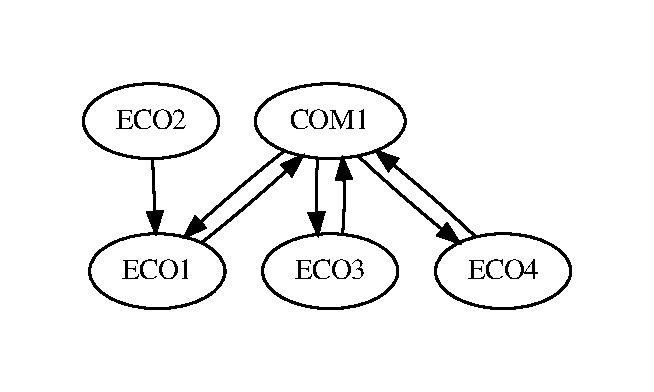
\includegraphics{M1.pdf}
\end{figure}

\subsubsection{Model 2}
Arguments include COM1, ECO1, ECO3, ECO4, but ECO2 changes to:
\begin{description}
	\item[ECO2'] [ ( scalingUp $→$ (buildingCosts $\land$ labourCosts $\land$ automationCosts) ) $→$ increasedCosts ] $→$ reducedEconomicBenefit
\end{description}

Logical contradictions are the same.

Attacks: see \cref{fig:m2}.
\begin{figure}
	\caption{Attacks resulting from model 2}
	\label{fig:m2}
	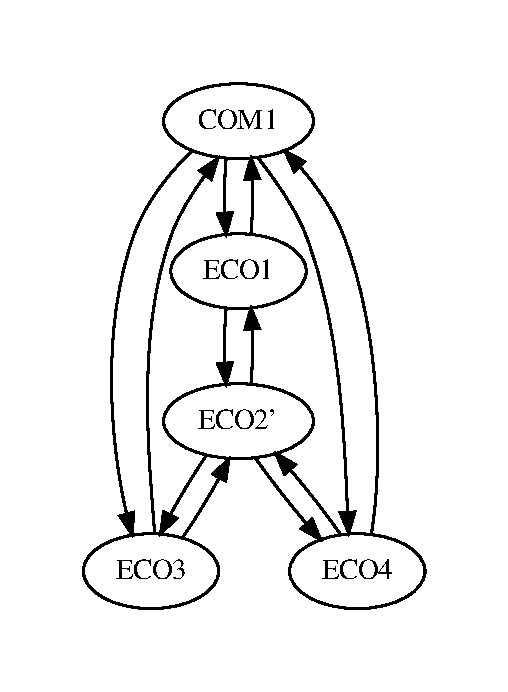
\includegraphics{M2.pdf}
\end{figure}

\subsection{General study}
Let $T$ be a set of possible texts in natural language and $p$ a procedure that transforms any text in $T$ into a set of undercut trees $\mathcal{U}$. Considering the classical logic approach first, we assume $p$ takes the following form: it first applies a set of possible interpretations of the text using a function $i$ to yield $\Delta, \Delta', …$, which are then used to produce undercut trees. Define $C$ as the classical logic approach defined above; applying $C$ to $i(t)$ thus results in a set of sets of undercut trees (one set for each $\Delta$).

For the conclusions to be non-trivial, we request that $\exists t \in T, \phi \in L(i(t)) \suchthat i(t) $ permits to deduce $\phi$ but $C(i(t))$ contains no tree with an undefeated root arguing for $\phi$. Here $L(i(t))$ denotes the set of formulas that can be formed using the atoms in $\cup i(t)$.

For the interpretations to be neutral (in the sense of making no assumption on the quality or content of the arguments in the text), we request that $i$ satisfies the following: $\forall t, \Delta \in i(t)$, $\Delta$ is closed under $¬¬$ (thus $\Phi \in \Delta ⇒ ¬¬\Phi \in \Delta$).
\footnote{Previously, but probably incorrectly, I requested for all $t$ that if $\exists \Delta \in i(t), \Phi \subseteq \Delta \suchthat MUS(\Phi)$, then $\exists \phi \in \Phi, \phi' \notin \Phi \suchthat MUS(\Phi \setminus \set{\phi} \cup \set{\phi'})$. $MUS(\Phi)$ means that $\Phi$ is a minimal unsatisfiable set.}

\begin{theorem}
	There exists no $p = C \circ i$ such that $i$ is neutral and $p$ has non-trivial conclusions.
\end{theorem}
Given a tree $(n, s)$ with $N = s[n]$ and $M \subseteq N$, define $D(M) = \set{S \subseteq N \suchthat s(M) \subseteq s^{-1}(S)}$ as the set of coalitions that attack all the attackers of $M$ (such a coalition is said to defend $M$). Say that $M$ is warranted iff for some finite sequence of the form $D_1 \in D(M), D_2 \in D(D_1), …, D_k \in D(D_{k - 1})$, we have $s(D_k) = \emptyset$.
\begin{lemma}
	A root is undefeated iff the singleton containing the root is warranted.
\end{lemma}

\subsection{More discussion}
\commentOCf{Contenu de cette section à reformuler ou effacer à terme…}

The assumption we want to discuss here is the following.
Many articles start with a postulated known attack relation or logic representation of arguments. It is natural to wonder where this information might come from, and we suppose, although this is seldom discussed explicitly, that the assumption is that it is more or less easy to obtain such relations from the natural language form in which arguments generally arise in the wild. 
The postulate that we want to argue against here is that by inspecting the arguments and using common sense, either the attack relation can be seen immediately, or a logical representation of the arguments can unambigiously be obtained, itself yielding a non-trivial attack structure by logical manipulation.
By non-trivial, we mean here that the structures that are obtained do permit, at least sometimes, to discriminate between a claim and its negation, even though both the claim and its negation can be deduced from arguments in the text. (Intuitively, we want to exclude cases of obtaining entirely symmetric conclusions.)

Accordingly, we focus on the case of arguments given under natural language. 

We make the following hypothesis of robustness against interpretion. The set of possible interpretations is $I$. If an interpretation leads to $\Delta$, and some argument in the DB says $\Phi$ and is attacked by $\Psi$, and it is possible to deduce, from the DB, using elements from $\Phi$ and $\Psi$, a counter-argument, then it is included in the set of interpretations.

Undoubtedly, some situations let one determine easily the attack relation, by simple appeal to an obvious consensus. In the classical textbook example of Alice saying that “it will rain tomorrow because the weather forecast on the BBC said so” and Bob replying that “it will not rain tomorrow because the weather forecast on Channel 4 said so”, the situation is clear, and a simple appeal to consensus permits to solve any doubt to the contrary: give these arguments to any two persons, and they will agree that these arguments attack each other. Such trivial situations, although being possibly adequate for illustrative purposes of technical definitions, are however hardly representative of the complexity of the debates that an argumentation framework must be able to tackle. It seems reasonable to demand of argumentation theory to help us think about debates involving subtle, complicated arguments. For example, a framework could claim to be able to help a medical doctor take a decision about which treatment to prescribe, or help an individual to choose which political party she will vote for.

Our main claim is that there is no neutral formal way to determine an attack relation that is not symmetric. In other words, obtaining a non-symmetric attack relation requires the analyst to adopt a position in the debate, in the sense of considering some claims as “winning” over others in a way that cannot be justified in purely formal terms.

First, note that one can always interpret “kindly” any argument, by filling in (considering as implicit) any supplementary claim that is required to make it work. To illustrate, assume John says: “because the apple detached from the tree, it fell on the ground”. The antecedent is not sufficient to bring the consequent: in case of storm, for example, the apple could detach from the tree and (temporarily) not fall on the ground. Depending on the circumstances of the speech, however, it might be perfectly reasonable to assume that John really meant: “because the apple detached from the tree and there was no storm on that day, it fell on the ground”. Indeed, if a required element in a reasoning is missing, it may be because it is an implicit assumption (that perhaps John knows is shared by the audience, hence does not consider useful to say). Now, interpreting kindly any argument will constantly lead to abstain from any conclusion: any argument that attacks any other will be attacked in return. Indeed, imagine someone says: “as there was storm on that day, the apple did in fact not fell on the ground”. Interpreting John’s text kindly, we would conclude that these arguments attack each other, and will not be able to conclude anything.

If we want to avoid this unfortunate consequence of extreme permissivism, we must restrict which attacks we (as modelers) we consider as “plausible”. In the famous Tweety example, we consider likely that the defeasible rule Bird(x) => Fly(x) is abusively used for building the argument that Bird(Tweety) and therefore Fly(Tweety), in a case where Tweety is a penguin; and we obtain a not too permissive model where the argument Penguin(Tweety) attacks the first one. But we could, again, conclude otherwise: if, unknown to the modeler, the person uttering the sentence in favor of Tweety flying is talking about an island where there are only birds that fly, then the use of the rule is authorized, and the person saying that Tweety is a Penguin must be mistaken. It is a choice of the modeler to conclude otherwise.

This shows that one will either be overly permissive, or need a trusted source of knowledge (that defines a hierarchy of claims by plausibility, say).

Another way to view this tension is to observe that we need to interpret what John says: we do not know what is missing from his reasoning because he did not realize some supplementary hypothesis was required (and therefore possibly obtained a mistaken conclusion), or because he thought it was sufficiently clear for the audience that the hypothesis was holding in the context of his speech.

More generally, using the scheme requires to add a priori knowledge, which is usually left implicit in the literature but is nonetheless required. Defeasible rule: A implies B. Explicit rule: A and X imply B. Attack: not X. But we might instead make the first speaker win the argument by instead being more kind to him and considering that the mere fact that he used the rule A implies B means that he implicitly thought it clear that X hold as well. (This kind hypothesis may seem reasonable in some contexts, such as when the speaker is an expert in the relevant domain.) Also, it could be that there is another way to complete the defeasible rule A implies B, by saying A and Y imply B. In that case, not(X) is uneffective against the first speaker. When the modeler considers that an argument attacks another one, and not conversely, she is inevitably taking a (possibly implicit) position in favor of some of the arguments.

We can rephrase this by saying that a first and important reason to not consider the attack relation known a priori is that considering it known a priori seems to require to assume that the attack relation is objective, thus in particular, that whether an argument attacks another one does not depend on who is listening, or on a choice of interpretation. The objectivity assumption permits to declare that an argument “truly” attacks another one, even though some given person may fail to realize it or may even believe the contrary. 

Real-life debates feature omissions and implicit statements. It may be fundamentally undetermined (and not simply unknown) which statements exactly have been omitted so as to connect an argument to what the debater has said previously. The debater himself may be hard pressed to explain it, if asked: we human being may not always form fully precise statements mentally before uttering them, or if we do, we do not necessarily have access to the precise version of the statements. A mathematician might “feel” that a proposition is true long before knowing how to prove it. A person may intuitively “see” how one argument supports or attacks another one without being able to fill in all the gaps and make it a precise reasoning. Or there may be multiple reasonings that allow to fill in the gaps, and the debater may erroneously think that they are just different ways of expressing the same idea; whereas it could be that one phrasing features a mistake in reasoning whereas another one does not. It is the norm with philosophers debating of complex ideas to consider multiple versions of their opponent’s claim, trying to interpret them “kindly”, that is, filling what they see as gaps in their opponent’s reasoning in ways that make their opponent’s view point as solid as possible (cite Denett). It seems hard to justify that one of these versions in particular would objectively be the right version. And if there are indeed multiple interpretations of a statement that correspond to multiple precise arguments, it seems unlikely that they all would lead to the same attack relation when considered within a set of related arguments. Therefore, in some interesting cases, the attack relation is not objectively determined.

Another important reason to not consider the attack relation known a priori relates to the understanding of the attack relation itself. 
Even when arguably “what the debater means objectively” is well defined, one may, in some applications, be interested in what some given listener understands from the debate, rather than by what the debater means. 
This is an important distinction in our context because the attack relation representing what the listener understands may differ from the one representing what the debater means.
The listener may not know the meaning of some words used by the debaters, or she may understand them differently than what the debaters have in mind. 
The listener may not have the deductive power to understand what could otherwise be considered a trivial implication of the argument. 
The listener may lack some required knowledge.

Translating natural language arguments into a logic language does not constitute a solution to these problems, as the problems exist, unchanged, at the level of translation. When there are multiple ways of interpreting some implicit information present in an argument (as intended by the debater, or as understood by the listener), the modeler must choose one when translating it in a formal, precise language, with the risk of introducing an arbitrary choice or losing neutrality.

A practical argument is that encoding the arguments logically require important expertise, which may be unavailable or cost too much.

\commentOC{To discuss: which points require examples? How complex (toy examples VS realistic examples)? Consider an example of a logic encoding with different conclusions?}

Practical studies showed that rejected arguments are not necessarily to be interpreted as non-receivable, but rather as rough ideas that need to be refined \cite{EJDP2018, Bourguet2013} and can serve as initial pillars of great importance for the construction of the argumentation system. Talk about obtaining judgements of individuals, …

\section{what if not known a priori?}
We just argued that it may be relevant or convenient to not assume we know the attack relation. In this section we provide some ideas of subject of studies that do not require this assumption, that pertains to computer science, and does not require advanced natural language processing capabilities.

(To be continued.)
We consider that what counts is what the receiver of the argument says and we propose to study several aspects related to this perspective: how to find decisive arguments in this sense; is this consensual; what are appropriate methods, statistical or others; what are the protocols that must be used to gather arguments; how can we test that every arguments that are possibly relevant have been considered?

\section{a sketch of a possible approach}
Let people come to a website and argue and indicate which arguments theirs answer, then confront this to the opinion of other visitors
\commentRT{Raccrocher Nicolas ici ?}

\section{Others}
We should decide whether to include some of these points in the text or adding sections about them or dropping them.
\begin{itemize}
	\item possibly, contrast with persuasion?
	\item link to explainable AI (should focus on decisive arguments), exploitation of weaknesses of will or sub-conscious behavioral patterns (youtube autoplay; nudge; anchoring) VS reflective arguments (advocacy), and the like? Link to deliberative democracy?
	\item review existing experimental work in FAT? Other related works? Philosophical approaches (Rawls, Habermas)?
\end{itemize}

%\bibliography{bibl}

\end{document}
